\documentclass[11pt,a4paper]{article}
\usepackage[utf8]{inputenc}
\usepackage{amsmath}
\usepackage{amsfonts}
\usepackage{amssymb}
\usepackage{parskip}
\usepackage{tikz}

\usetikzlibrary{arrows,positioning} 
\tikzset{
    %Define standard arrow tip
    >=stealth',
    %Define style for boxes
    punkt/.style={
           rectangle,
           rounded corners,
           draw=black, very thick,
           text width=6.5em,
           minimum height=2em,
           text centered},
    % Define arrow style
    pil/.style={
           ->,
           thick,
           shorten <=2pt,
           shorten >=2pt,}
}

\author{Finnian Lattimore}
\title{A short introduction to causal inference}
\begin{document}

\section{Abstract}
wide applicability makes it an inherently multidiciplinary field, economics, social science, philosophy, statistics and more recently, computer science.

cross-world independence cannot be determined experimentally - thus not subject to scientific scrutiny. The problem is if we are doing induction, we have already made assumptions not subject to scientific scrutiny. 
\section*{Introduction}



The notion of causality is deeply tied to questions about actions and interventions. Does high blood pressure cause heart attack – or are the two merely associated through a third causal factor? Would taking action to reduce blood pressure reduce the risk of heart attack? Sometimes these questions can be resolved by direct experiment, however this may be prohibitively expensive, ethically unconscionable or technically impossible. For these cases the question arises, can we infer the consequences of action from purely observational data? Without making any assumptions, this is impossible. The fundamental problem of causal inference can be illustrated by a simple diagram (Figure XXX). 

Classical statistics deals with the question; Given samples from an unknown distribution, what can we say about that distribution. Causal inference asks; Given samples from an unknown distribution, what can be inferred about the distribution after I take some action? Without making any assumptions about how the action could effect the distribution, that question is unanswerable no matter how many samples are available. 

There are two somewhat distinct problems commonly referred to as causal inference. The first deals with estimating causal effects where the structure of the relationships between variables is considered given by theory or other prior knowledge. This form of causal inference is prevalent, often implicitly, in almost every area of scientific research and techniques to address it have been developed in parallel in economics \cite{Heckman}, physcology \cite{Campbell}, statistics \cite{Rubin} and computer science \cite{Pearl}. 

The second and more difficult problem is to infer the structure of the causal relationships between variables. Any causal inference requires either experiment or assumptions, thus determining causal structure from observational data is impossible without some assumptions. However, recent research, XXXX, XXXX,XXXX has demonstrated that some aspects of causal structure can be identified from very general assumptions.


\section*{Defining Causality}

In order to study causality, we need clearer definition of what we are talking about. There are a number of different approaches to defining causality. 

\subsection*{The Neyman-Rubin model}


The Neyman-Rubin model defines causality in terms of potential outcomes, or counterfactuals. It was developed from the starting point of randomized experiment and shares much of this terminology. A causal effect is defined as the difference in outcome for the same subject under different possible treatments. Expressed mathematically, assume we wish to understand the causal effect of a variable we will call $T$ (for treatment) on an outcome variable $Y$. For simplicity and consistency with the majority of the literature, I will assume $T$ is a discrete, binary variable. The levels of $T$ are often referred to as active ($T=1$) and control ($T=0$). for an individual unit (person, location, etc) $i$  that could be assigned a value of $T$, the individual causal effect $e_{i}$ of $T=active$ relative to $T=control$ on outcome $Y$ is defined by:
\begin{equation}
\label{eq:ICE}
\tau_{i} = Y_{i}(T=active)-Y_{i}(T=control)
\end{equation}
These can not both be directly measured, since a single unit is can only be exposed to one of the two options. This is what Rubin calls the fundamental problem of causality. The problem can be resolved if you can assume based on prior knowledge that all units are identical or that units will revert exactly to their initial state some time after treatment. This type of assumption often holds to a good approximation in the natural sciences, and explains why researchers in these fields tend not to be concerned with causal theory.  

Rather than trying to estimate individual causal effects, one can focus on the average causal effect, defined as:
\begin{equation}
\label{eq:ACE}
\tau = E[Y_{i}|T=active] - E[Y_{i}|T=control]
\end{equation}
It is essential to understand that the averages in equation (\ref{eq:ACE}) are over both potential outcomes for all the units in the population regardless of which treatment they actually received. What can directly be measured, in an experimental or observational study, is the difference in means of the observed outcomes for the treatment and control groups, sometimes referred to as the \textit{prima facie causal effect}. :
\begin{equation}
\label{eq:observed_outcome_mean_difference}
S^{*} = E[Y_{j: j \in treated}|T = active] - E[Y_{k: k \in control}|T = control]
\end{equation}
In general, the average causal effect (\ref{eq:ACE}) and the observed difference in means (\ref{eq:observed_outcome_mean_difference}) will not be equal. However, if the assignment of units to treatment is random, then in the limit of large numbers of units the two will converge (Rubin). This formalizes the case for using randomized experiments to answer causal questions. It is interesting to note that this analysis relies on properties of the mean operator. If one is interested in other measures of the distribution of individual causal effects, or the form of the distribution as a whole, then randomization is less powerful (Heckman).

The Neyman-Rubin model extends to observational studies by careful modelling of the mechanism by which units are assigned to treatments. In particular, propensity scores, the most widely used technique arising from the Neyman-Rubin framework, stem from theAt heart, the Rubin Causal Framework is primarily a definition of causality in terms of counterfactuals, along with the recomendation to conceptualize inference from observational studies in terms of trying to frame it as random experiment. Quote XXXX. idea that if one could stratify on all variables that effected assignment to treatment, then within each strata, the prima facie causal effect would equal the average causal effect. The rest of the technique is just a clever way to approximate this when covariates are continuous or high dimensional such that stratification is not possible.   

Assumptions, ignorability, strong ignorability, SUTVA.

At heart, the Rubin Causal Framework is primarily a definition of causality in terms of counterfactuals, along with the recomendation to conceptualize inference from observational studies in terms of trying to frame it as random experiment. Quote XXXX.


\subsection*{Structural Equation Models}

A (causal) structural equation model is a set of $n$ equations of the form:
\begin{equation}
\label{eq:struct_eq_mod_definition}At heart, the Rubin Causal Framework is primarily a definition of causality in terms of counterfactuals, along with the recomendation to conceptualize inference from observational studies in terms of trying to frame it as random experiment. Quote XXXX.
x_{i} = f_{i}(pa_{i},\epsilon_{i})
\end{equation}

where $X = \{x_{1}...x_{n}\}$ are variables, $f_{i} \in \{f_{1}...f_{n}\}$ are deterministic functions, $pa_{i}$ stands for the set of variables that directly effect $x_{i}$ and $\epsilon_{i}$ represents noise introduced by not incorporating all sources of variation as separate variables. The noise terms are, by construction, mutually independent. Any variables that directly effect more than one variable in the model must be included in $X$. 

Structural equation models can be represented graphically as a network. Each node represents a variable and its associated deterministic function and a link $x_{i}->x_{j}$ indicates $x_{i}$ causes $x_{j}$. 





A causal inference perspective on the problem of granting bail.

Consider the following, greatly simplified, model of the bail process: People arrested on suspicion of committing a crime are brought before a judge, who decides if they should be granted bail (released into the community) or remanded in custody until they face court. The court must balance the rights of a person presumed innocent against the risk they fail to appear at a hearing, interfere with a witness or commit some other offence if released. For simplicity, we group all these issues into a single concept of 'bad behaviour'. The problem is now to decide, based on the available evidence, if a person is a high or low risk of bad behaviour.  

Estimating risk is difficult for humans to do accurately, which motivates the application of machine learning and statistical techniques. Additionally, a computer algorithm can be designed to avoid particular forms of bias, for example based on race or physical appearance. The problem appears to be standard binary classification, suggesting that it should be straightforward to apply machine learning techniques and assess if they are better at predicting who will break bail than judges. However this ignores the way in which the data, on which a machine learning algorithm could be trained, was generated. 

Image we have a large data set on what happened to people released on bail. For each person we have a set of variables, we will denote as Z, describing their personal attributes and the crime they are accused of. We also have a binary variable Y that specifies if they behaved badly or not. We train our machine learning algorithm on a subset of the data and then test on the remainder to see how it did and get out the following confusion matrix. 



they are accused of and a binary variable 

 age, sex, prior history, shoe size, 












A few different possible causal models to consider 

Estimation of the probability of bad behaviour is central to the decision, motivating the use of machine learning provide a predictive model.  

he fact that the decition to grant bail is substantially based on the risk, that is probability, that a person will behave in a particular way motivates applying machine learning and statistical technqiues. Such techniques be additionally justified by the possibility that they can be designed to avoid particular bias - for example on race, or physical appearance. But is the problem fundamentally statistical?

What bounds?

Under what circumstances could we empircally show statistical techniques were fairer, reduced risk. etc. 



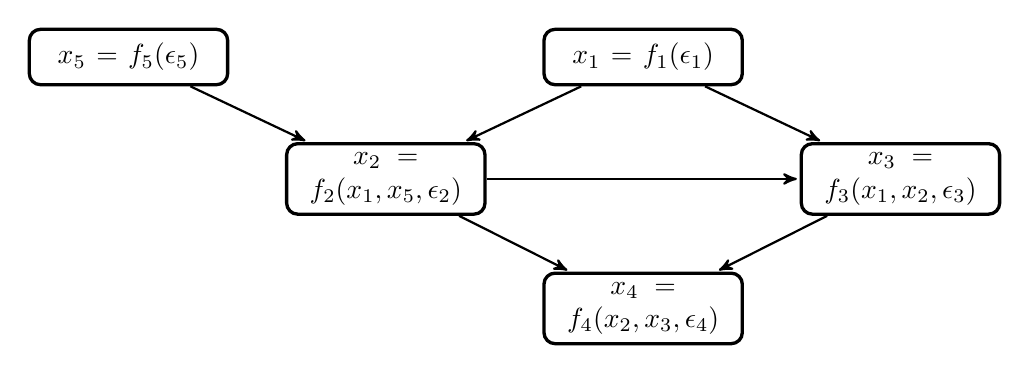
\begin{tikzpicture}[->,>=stealth',shorten >=1pt,auto,node distance=1cm,
  thick,main node/.style={punkt}]

\node[main node](1){$x_{1} = f_{1}(\epsilon_{1})$};
\node[main node, below left=of 1](2){$x_{2} = f_{2}(x_{1},x_{5},\epsilon_{2})$}; 
\node[main node, below right=of 1](3){$x_{3} = f_{3}(x_{1},x_{2},\epsilon_{3})$};
\node[main node, below right= of 2](4){$x_{4}=f_{4}(x_{2},x_{3},\epsilon_{4})$};
\node[main node, above left=of 2](5){$x_{5} = f_{5}(\epsilon_{5}$)};

 \path[every node/.style={font=\sffamily\small}]
    (1) edge node {} (3)
        edge node {} (2)        
    (2) edge node {} (4)
    	edge node {} (3)        
    (3) edge node {} (4)
    (5) edge node {} (2);
	

  
\end{tikzpicture}


Structural are ubiquitous across economics and social sciences. The causality comes from what we define the equations or links to mean. A causal structural equation model clearly specifies our assumptions on the causal structure of the problem. Missing links in the network (or equivalently, excluding a variable from the set $pa_{i}$ represents an assumption that x does not directly cause y). Asserting a structural equation model for a given problem cleanly encodes a set of assumptions. 

Interventions in structural equation models correspond to external modification of functions and variable distributions. The do opperator.   

Extensively applied and causaly interpreted in economics - exemplified by Wright 1921, Haavelmo 1943 and more recently Heckman. Generally with additional assumptions that the functions are linear and the noise additive. 

Counterfactuals can be derived from structual models.

\subsection*{Causal Graphical Networks}

Graphical models (Pearl)
Causal Bayes nets are a subset of structural equation models for those who have philosophical objections to counterfactuals. 
Defined in terms of interventional distributions. 

Potential outcomes and structural equation models allow statements about counterfactuals. Causal Bayes nets are 


\subsection*{Differences, similarities and controversies}



Remarkably for models developed relatively independently in fields with very different approaches and problems, the models we have discussed are definitionally (almost) equivalent. However, the practical guidance given by their proponents on applications differs. This has led to confusion and controversy.  

The key difference between Rubin and Pearl is that Rubin does not make explicit how you decide which variables one should satisfy/condition on/include in a propensity score. In some cases Rubin has implied one should condition on as many variables as possible "quote". Using a graphical framework it is easy to demonstrate that it is possible to increase the bias in a causal estimate by conditioning on certain variables, for example, a collider.  XXXX gives some plausible examples of real cases where this could occur. The correct answer to which variables should be conditioned on relies on making some assumptions about the plausibility of the structural role played by that variable in the problem. It is possible that certain structures are more prevalent in nature or within particular research fields. Similarly for particular distributions and functional relations between them, conditioning on a variable that should have been excluded could do less harm than not conditioning on one that should have been included. (binary variable thing). However, such justifications for conditioning on a variable where you have 'no idea' about its true causal structure should be explicitly stated. Alternatively one could estimate the causal effect for each structural model possible with in the assumptions you were willing to make incorporate the resulting uncertainty into the reported effect.   

Pearls work focuses on the large sample limit and non-parametric inference, and providing very clear theory. Rubin's papers contain a series of more practical examples, and advice and techniques, in particular propensity scores, that are useful for applied work.

Propensity scores are a purely statistical concept. They can be calculated directly from joint distributions over variables and do not contain any extra-statistical or causal information. However, they address a problem that is commonly encountered in practical causal inference with finite data: how do you condition on a continuous or high-dimensional set of variables? 

Perhaps as a consequence of this difference in focus, Rubins work has been widely cited in applied research in XXXX, as opposed to Pearl (use some citiation data to check that). One provides clear, simple theoretical method for describing what assumptions one must make, which variables should be conditioned on. The other, a notation that can elegently capture the what if types of queries that humans often phrase as causal queries and propensity scores.

Also the focus on treatment assigment ignores other causal inference techniques such as instrumental variables that can be represented and described by structural equation models. 

Rubin's focus on expectation values may contribute to its empirical success/use vs Pearls work is more general but may be more sensitive to sampling issues. More concrete, less general complete theory. Way in which the material is presented may be more accessible to practitioners. 

warnings not to adjust for post-exposure variables (mentioned in Greenland  Robins 2009). Reference Cox DR: Planning of Experiments New York City: John Wiley and Sons
Inc; 1958.

Is it important to only consider interventions on variables that could 'potentially be modified'? : Epidemiologic measures and policy formulation:
lessons from potential outcomes,
Invited commentary: hypothetical interventions
to define causal effects--afterthought or prerequisite?



\section*{Estimating Causal Effects}

If you are using the do-calculus to estimate causal effects, the assumptions you are effectively making are the weak ones preferred by Robins, et al. Ie for any problem involving only interventional queries, the answer will be the same if you use weak or strong ignorablility. 

Firstly, estimating the magnitude and direction of causal effects where the structure but not functional form of the relationships is known and secondly inferring the structure of cause and effect between variables. 

Firstly the problem of estimating causal effects where the structure of the relationships between variables is known. 

1) You assume you already know the causal structure of a set of variables and the goal is to infer the value of a given causal effect, or in other words the consequence of an intervention. Assuming the structure means you could draw a network of the variables with arrows from causes to effects. You can allow for variables you cannot measure but you still need to draw them into the network and specify how they are linked to observed variables.

In the large sample limit, this problem is solved. The do calculus (Pearl 2000) tells you when the problem is identifiable and if it is, gives a formula to calculate the causal effect. A causal effect that is not identifiable under the do calculus cannot be estimated purely from observational data, no matter how many samples you have, without making additional assumptions. Some problems that are not identifiable can still be solved if you are additionally willing to make parametric assumptions about the form of the distributions of variables and the functional relationships between them.

Where the causal effect is not non-parametrically identified, you may still be able to bound it. 


An extremely short summary of Pearl on this matter. 1) Assume causality defined by a SEM (or a causal Bayes network). 2) This allows us to view interventions as modifications to the graph. 3) The 3 do-calculus rules can be derived from d-seperation on the modified graph. 4) These rules are complete. They can be used to determine if a interventional query is non-parametrically identifiable and if so, what the formula for calculating it is. 5) The back door and front door criterion are sufficient but, not necessary, for causal identifiability. They are handy shortcuts to applying the full do-calculus algorithm as they cover many types of causal structure. Also, back door lines up with when one can calculate causal effect by conditioning. Front door corresponds to identifying by sequentially cacluating other effects. A generlizing sufficient condition for identifying P(y|do(x)) is that there exists no path consisting of only bidirected arcs between X and any of its direct children. Tian  Pearl 2002a 



2) Given only observational data on a set of variables and infer the causal structure between those variables. This is a much harder problem, perhaps surprisingly, some aspects of causal structure can non the less be inferred with fairly broad, Occum's Razor type assumptions. 

Frameworks. Structural Equation Models SEM is where its at …

We will begin our consideration of causal frameworks with regard to the first question. 

Holland “For causal inference, it is critical that each unit be potentially exposable to any one of the causes. As an example, the schooling a student receives can be a cause, in our sense, of the students performance on a test, whereas the student's race or gender cannot” This seems like a major draw back … Rubin would see this as still a meaningful causal effect. 

First ingredient – a definition of causality. 

Rubin defines causal effects in terms of counterfactuals on individual units. But the quantity actually estimated is the average causal effect across all the units. Rubin demonstrates that a classic randomized experiment gives an unbiased estimate of this quantity. Rubin – design experiments to approximate randomized experiments.

2 key parts – definition in of causal effects in terms of counterfactual statement about potential outcomes. 2) Explicit description/modelling of the assignment process that determines which units received which treatments. Rubin 2008

“The assignment mechanism gives the conditional probability of each vector of assignments given the covariates and the potential outcomes” ,”we attempt to assemble data with 
enough covariates that it becomes plausible (or initially arguable) that the 
unknown assignment mechanism is unconfounded given these covariates” 
Rubin 2007 Handbook of stats

The definition of causality in term of counterfactuals is consistent with the graphical model.


The transport safety causality study seems to be confused about the assumptions required for potential outcome modelling. 


\section*{Random Thoughts}
Gelmnans objections to causal structure learning - no true 0's. Should not be nessessary to think in terms of conditional independencies to do causal inference. Models are styalized -> likely everything comes out linked to everything. I guess it is a very testing based approach... scoring or averaging might appeal more. 

Accepting the limitations of science. (or statistical inference). Note parallel between requirement for assumption in statistics (due to the no-free lunch theorem) and the requirement for assumption in causal inference.

Another question, why does assuming things are linear (even when we know they are not) seem to work so well. Are many relationships in the world linear or roughly linear over the observed domain? Similarly the default assumption is independence of effect. 

Practical implications - just how much data is required to do particular sets of tests. When do you have enough data to do things non-parametrically? When could you test conditional independencies. Is there a rule of thumb that would tell you (say you were willing to assume Markovian model) how many data points would be required to do reasonable inference - or to give confidence intervals on the results. 

What other assumptions could you use to narrow down confidence bounds (what about if you were willing to rank variables/links by their magnitude of effects, or too specify if the effect would be positive or negative. 

could you build something that calculated this for simple models (ie discrete ones ...)

What field of real data might find application (with some form of ability to varify) ... (why are longitudanal studies important ... Longitudanal study of Australian Children, Census data, Neuron firing data, genetic data, 

How can we combine with reinforcement learning approaches ... if we get additional information back when we run an experiment, can we use causal inference theory to help tell us which experiment we should do next? What is the simplest (theoretical) model I can come up with that would allow exploration of this?

The whole idea of random variables in this way is not 'true'. If we can break things down enough you end up with quantum theory which, although contains randomness at a fundamental level, this randomness does not obey the standard rules of probability. The way we group events together and call things variables is clearly an approximation, but a powerful one. Relates to things like IID assumption...


When is dislike of black boxes justified. How does this relate to causality? What possible solutions are there to this (ie running multiple models in parralel and report when they diverge). Covariate shift - but you only care about shifts in covariates that effect the predicted outcome. Goal - find a bunch of predictive models that are diverse (in terms of the variables they rely on) but give 'high' predictive accuracy. 

When do we not really want a causal model? Is it really that we always do, but in some situations, predictive models place strong bounds on causal queries?




\section*{Inferring Causal Structure}
\end{document}